% divergence test
% modules -> table with short descriptions
%permutation of matrix ->orientation
%change from local to global coordinates
%rotation
%adaptivity
\section{Implementation}



\subsection{Subsection}
Cite like this\cite{succi}.

If you want to include figures, incorporate them as for example Fig. \ref{fig:lbm}.

\begin{figure}[h!]%
 	\begin{center}%
 		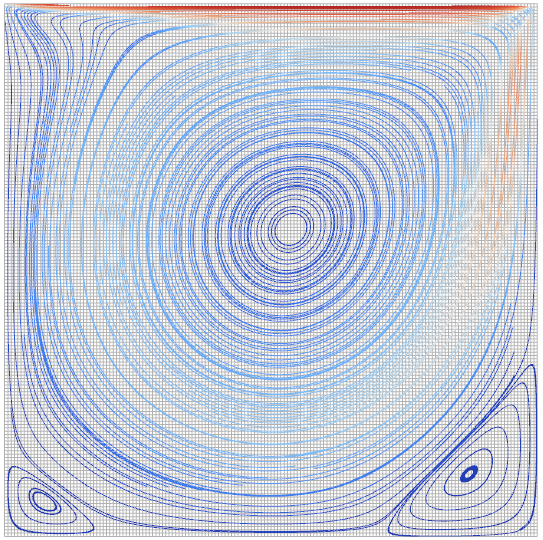
\includegraphics[scale=0.5]{figure1.png}%
 		\caption{Tree}\label{fig:lbm}%
 	\end{center}%
\end{figure}

Tables (cf. Tab. \ref{tab:example}) can also be incorporated.
\begin{table}[h]%
 	\begin{center}%
		\caption{Exampletable}\label{tab:example}%
	 	\begin{tabular}{c|c}%
 			col1 & Col2\\
 			\hline
 			0 & 1\\
 		\end{tabular}%
 	\end{center}%
\end{table}
